\chapter{\label{ch:ch02}ПРАКТИЧЕСКАЯ ЧАСТЬ}

Программа написана на определённых конфигурациях и версиях вспомогательных программ:

\begin{enumerate}
\item Операционная система windows 7
\item Среда программирования Python: версия 3.7.2 (64-bit)
\item Библиотека tkinter: версия 8.6
\item Текстовый редактор Geany: версия 1.38
\end{enumerate}

\section{\label{sec:ch01/sec01}Задумка и основные функции}

Моей программой должна стать игра "Танчики". Это должно быть, в первую очередь, игровое поле, сосотоящее из блоков (кирпичных и железных стен). В ней игроку предстоит перемещаться по игровом полю и побеждать вражеские танки, за уничтожение танка начисляются очки, которые формируют счет игрока. Игра продолжается до тех пор, пока танк игрока не будет уничтожен.

Само игровое поле будет иметь возможность редактировать размер, состав и расположение объектов на ней, при это будет менять и размер окна программы.

\section{\label{sec:ch01/sec02}Структура программы}

В данном разделе будут описаны все составляющие игры.

\subsection{\label{sec:ch01/sec03/sub01}Игровое меню}

Игровое меню - это то, с чего начинается программа сразу после запуска. Это будет окно размером 800*600 пикселей, содержащий на себе название игры и список кнопок, по которым будет происходить переход.

\subsection{\label{sec:ch01/sec03/sub02}Настройки}

Один из переходов в программе, к которой можно перейти из главного меню. Он будет содержать такие опции, как возможность создать свое собственное поле с желаемыми размерами и разместить на них игровые объекты (кирпичные, железные блоки) либо выбрать поле по умолчанию.

\subsection{\label{sec:ch01/sec03/sub03}Окно "О разработчике"}

Это окно будет выводиться по нажатии кнопки "Разработчик" в главном меню. Оно будет содержать информацию Фамилии, Имени и группы студента, разрвботавшего данную программу.

\subsection{\label{sec:ch01/sec03/sub04}Игровое поле}

Это онсновной цикл в программе, в котором на холсте (окне игры) будут размещаться игровые объекты, происходить взаимодействия между объектами, игроку будет предоставлено управление с клавиатуры.

Размер окна в этом разделе будет варьироваться от количества блоков игрового поля в ширину и высоту (количество блоков * размер блока) (но не равны нулю, само собой).

\section{\label{sec:ch02/sec03}Написание кода}
Основная структура:

Программа будет состоять из нескольких файлов, каждый из которых представляет собой отдельный раздел (за исключением файла config.py)

Главное меню:

Созадается основной файл main.py, с которого и будет осуществляться запуск програмы. Начинаем с разработки главного меню. Создается окно, дается название, задается фиксированный размер 800x600 и центральное положение (далее о центральном положении не будет упоминаний, т.к. это выполняется для всех окон по умолчанию). Tkinter позволяет очень просто разместить виджеты в любой точке рабочего окна. Размещены 4 кнопки друг под другом (с соответствующими заголовками). Они все будут выполнять функции, которые представляют собой открытия дочерних окон и работы в них.

Уже на этом этапе потребуется создать дополнительный файл config.py. Его задачей является хранения констант для возможности быстрого доступа, например в программе часто будет фигурировать размер блока, возможность регулировать параметры игры: частота кадров, скорость игрока, врагов и снарядов.

Об игре:

Как уже сказано ранее, этот раздел является функцией, которая открывает дочернее окно под названием about, которое, в свою очередь, находится в отдельном файле about. Все, что оно должно делать, так это выводить текст с информацией о названии, управлении и авторе. Выход из раздела будет осуществлен нажатием на крестик окна.

Игровой процесс:

Код самой игры расположен в файле game. Игровой процесс, по сути, является функцией под названием main. В начале этой функции идет процесс подготовки к игре, который включает в себя следующий алгоритм:
\begin{itemize}
\item Открытие файла map.txt (файл, содержащий данные о размере и расположении объектов на поле).
\item определение её размеров, открытие окна с вычисленными размерами.
\item Объявление 4-х классов (о которых будет далее).
    \begin{itemize}
    \item Функция Bullet:

    Эта функция отвечает за отрисовку движение и взаимодействие всех снарядов внутри игрового процесса.
    
    Каждый объект при создании имеет инициализацию. Объект добавляется в список всех снарядов (bullets), ему даются начальные координаты x и y, направления движения vx и vy, определяется владелец снаряда ouner и рисуется сам снаряд на холсте game\_sc методом create\_oval.

    Метод update класса Bullet выполняет роль логики для движения и столновения снарядов. Каждый цикл метода update продвигает снаряд на определённые координаты (x/y=x/y+vx/vy) и методом move холста game\_sc перерисовывается в новых координатах. Далее идёт проверка на столкновения с краями поля и стенами
    
    Противники: являются объектом класса Enemies. У них есть метод инициализации в котором:  перемешение основано на модели случайно блуждающей точки из книги Ю.Тарасевича "Математическое и компьютерное моделирование. Вводный курс"~\cite{book-math-mod}. Появление объекта класса
    \end{itemize}
\item объявление 2-х функций.
    \begin{itemize}
    \item Функция случайной генерации врагов (enemy\_spawn). Она начинается с того, что создается список mass размером map\_width * map\_height и заполняется нулями. Затем при помощи логической переменной block\_free координаты всех объектов на поле проверяются на наличие этих объектов на каком-то блоке. Если таковые нашлись, то ячейка списка mass в остановленной координате сохраняет значение 0 и значение 1 в другом случае.

    Она определена независимо от класса Enemy, так как её вызов обратился бы к существующему обьекту класса, который должен быть создан, что вызовет противоречие и, вследствие, ошибку.
    \item Функция cooldown содержит единственную строку, которая обнуляет переменную shotTimer объекта player. Она вызывается при помощи метода after, чтобы осуществить функцию задержки выстрела. После выполнения этой функции задержка пропадает и позволяет игроку совершить выстрел.
    \end{itemize}
\item загрузка необходимых изображений. В них входят:
    \begin{itemize}
    \item Изображения блоков (brick - картинка кирпичной стены, armor - картинка непробиваемой стены).
    \item Изобржения игрока (tank - список из 4 картинок одного зелёного танка в 4 различных направлениях)
    \item Изображения врага (аналогично с изображениями игрока, но цвет танка красный)
    \item Изображения взрыва (bang - список из 3 изображений последовательно анимируемого взрыва)
    \item Изображение для визуального интерфейса (HUD), дающий игроку знать, какое количество жизней у него в запасе (lives).
    \end{itemize}
\item Расположение на окне 2-х холстов (один (interface) для отображения интерфейса, второй (game\_sc) для отображения игрового поля).
\begin{figure}[h]
    \centering
    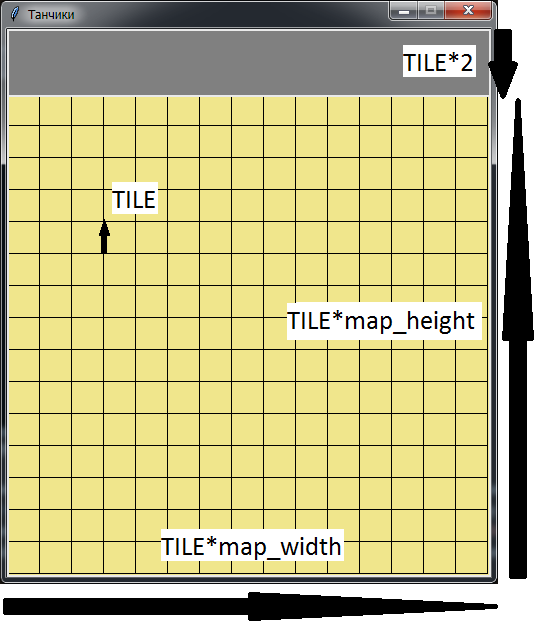
\includegraphics[width=0.5\textwidth]{./images/image1.png}
    \caption{\centering\label{fig:example05}Размещение холстов на игровом окне с размерами.}
\end{figure}

Холсты на окне размещаются в определённых размерах. Тот размер в блоках, что задаётся для игрового поля, является количество блоков, умноженные на длину одного блока (TILE). Панель интерфейса  расположена над игровым полем. Для неё выделено два блока в высоту Для размещения на нём количества жизней игрока и количество очков, начисляемые за уничтожение врагов. 
\item Заполнение холста game\_sc игровыми объектами. Имеется в виду расстановка кирпичных/непробиваемых блоков и места расположения игрока.
\begin{figure}[h]
    \centering
    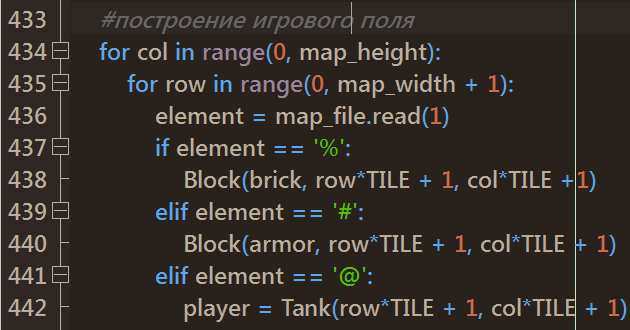
\includegraphics[width=0.5\textwidth]{./images/image2.png}
    \caption{\centering\label{fig:example05}Алгоритм размещения блоков и игрока на поле.}
\end{figure}

Это выполняется следующим образом: по вычисленным количествам блоков в ширину и длину выполняется двойной цикл for, который присваивает временной переменной прочтённый из файла map.txt символ, а затем, в зависимости от полученного символа выбирается установить вид блока на тех координатах, на которых в данный момент выполняется цикл.
\item Размещение на холсте interface надписи "Счет:", числа, обозначающего значение счета и кол-ва жизней игрока. Все они размещены с помощью виджета Label.
\item Циклом с пятью повторениями создание 5 врагов функцией enemy\_spawn.
\item Назначение функций движения игрока на клавиши. Функция move класса Tank назначается на нажатие любой клавиши клавиатуры "<Key>" (а уже внутри самой функции условия отсеивают нажатия конкретных клавиш), остановка движения функции stop определены на отпускание клавиш "<KeyRelease>", функция стрельбы игрока shoot назначена на нажатие кнопки пробела "<space>".
\item Объявление функции game. Это основной цикл игры, который за одну итерацию проходит по всем врагам, снарядам и игроку, чтобы выполнить однородный для всех объектов метод update. Чтобы возобновлять врагов после уничтожения и добавлять очки, применяется исловие на проверку длины списка врагов, в данном случае эта длина равна 4 и если окажется на один танк меньше (засчитано уничтожение), то будет переменная title\_score возрастет на 100 и появится новый враг посредством функции enemy\_spawn. Завершение игры должно произойти, когда кол-во жизней игрока станет равным 0, поэтому предлается следующая реализация функции game: метод after холста game\_sc, выполняя функцию game\_sc с очень маленьким промежутком (с задержкой в переменную FPS), создает эффект анимации. Из-за этого выполнение функции game становится бесконечным. Чтобы этого избежать, внутри функции game добавляется условие равенства жизней игрока нулю, и в таком случае предлагается выйти из цикла или подготовить игру к завершению.
\end{itemize}

\section{\label{sec:ch02/sec04}Тестирование}
Тестирование проводилось на следующем ПО:
\begin{enumerate}
\item Windows 7
\item Linux Debian
\item Текстовый редактор Geany: версия 1.38
\end{enumerate}
Первый запуск программы вывел ошибку. Причина: отсутствие некоторых подключенных библиотек в некоторых файлах. Программа соответствует задуманной структуре.
\begin{figure}[h]
    \centering
    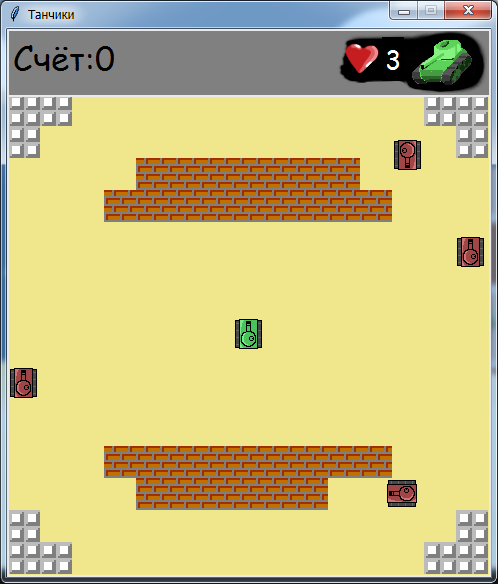
\includegraphics[width=0.5\textwidth]{./images/game_process.png}
    \caption{\centering\label{fig:example05}Итоговый вид игрового процесса.}
\end{figure}